% ======================================================================
% The Art of Solving Thermodynamics Problems -- RP's Method
% A self-contained prose companion to the two-video series.
% RPGroup @ Monash -- MMA2003 Thermofluids.
% ======================================================================
\documentclass[11pt,a4paper]{article}

\usepackage[a4paper,margin=2.4cm]{geometry}
\usepackage{parskip}
\usepackage{amsmath,amssymb}
\usepackage{bm}
\usepackage{array}
\usepackage{enumitem}
\usepackage{titlesec}
\usepackage{xcolor}
\usepackage{tikz}
\usetikzlibrary{arrows.meta,positioning,calc,decorations.markings,shapes.geometric}
\usepackage[colorlinks=true,linkcolor=monashred,urlcolor=monashred,
  pdftitle={The Art of Solving Thermodynamics Problems -- RP's Method},
  pdfauthor={Prabhakar Ranganathan}]{hyperref}

% ---- colours, matching the videos and the instructor solutions -------
\definecolor{monashred}{HTML}{C82506}
\definecolor{stateblue}{HTML}{1F5FBF}
\definecolor{procred}{HTML}{C82506}
\definecolor{tfgreen}{HTML}{1B6B3A}
\definecolor{extindigo}{HTML}{3F3A8C}
\definecolor{stmtgray}{gray}{0.5}

\newcommand{\stinfo}[1]{\textcolor{stateblue}{#1}}
\newcommand{\prinfo}[1]{\textcolor{procred}{#1}}
\newcommand{\Dg}[1]{$#1$\,{\scriptsize\textcolor{gray}{(given)}}}
\newcommand{\Dp}[1]{\textcolor{procred}{$#1$\,{\scriptsize(process)}}}
\newcommand{\De}[1]{\textcolor{stateblue}{$#1$\,{\scriptsize(EoS)}}}
\newcommand{\mcube}{{m\textsuperscript{3}}}
\newcommand{\degC}{{$^\circ$C}}
\newcommand{\cv}{c_{v}}
\newcommand{\cp}{c_{p}}
\newcommand{\wb}{w_{b}}

% ---- arrow-diagram + P-v TikZ styles (from the instructor solutions) -
\tikzset{
  pa/.style={-{Stealth[length=2.4mm]}, thick, procred},
  pvc/.style={procred, thick, postaction={decorate},
              decoration={markings, mark=at position 0.55 with {\arrow{Stealth[length=1.8mm]}}}},
  pvdot/.style={circle, fill=stateblue, inner sep=1.1pt},
  scir/.style={circle, fill=procred, text=white, font=\bfseries, inner sep=0pt,
               minimum size=6.5mm},
}

\titleformat{\section}{\large\bfseries\color{monashred}}{\thesection.}{0.5em}{}
\titleformat{\subsection}{\normalsize\bfseries}{\thesubsection}{0.5em}{}
\titlespacing*{\section}{0pt}{1.4em}{0.4em}

% ---- a light framing box ---------------------------------------------
\newcommand{\asidewidth}{\dimexpr\linewidth-20pt\relax}
\newenvironment{aside}[1]
  {\par\medskip\noindent\begin{tikzpicture}\node[draw=#1, fill=#1!5,
      rounded corners, inner sep=8pt, text width=\asidewidth, align=left]
      \bgroup\small}
  {\egroup;\end{tikzpicture}\par\medskip}

\begin{document}

\begin{center}
{\LARGE\bfseries\color{monashred} The Art of Solving Thermodynamics Problems}\\[4pt]
{\large RP's Method \textemdash{} a disciplined way to plan your attack}\\[8pt]
{\small Prabhakar Ranganathan \textbullet{} RPGroup, Monash University \textbullet{}
companion to the two-part video series}
\end{center}

\begin{aside}{extindigo}
\textbf{RP's method} This note sets out \emph{one} way to plan a
thermodynamics problem \textemdash{} the way I teach it. It is not the only correct
way, but shares shares its foundations with the worked examples you will
see elsewhere in the unit: the same first law, the same sign convention (heat in
and work out positive), the same distinction between \emph{state properties}
($P$, $T$, $v$, $u$) and \emph{process variables} ($q$, $w$), and the same
discipline of stating assumptions before computing. What this method adds is a
single organiser \textemdash{} the \textbf{arrow diagram} \textemdash{} that makes
the plan visible on the page before any number is worked. 
\end{aside}

% ======================================================================
\section{Why bother}

Engineering design and innovation are, at heart, the solving of complex puzzles.
A sudoku is a small, familiar example: you are handed a few numbers and a short
list of rules, and from those you deduce, square by square, everything left
blank. A thermodynamics problem is the same. You are given a few
properties, you know a fixed set of physical rules, and your task is to work out
everything else. Fundamentally, sudok puzzles, or geometry theorems, or thermodynamics problems are all exercises in deductive logic.

Every puzzle of this kind gives way to the same three moves:

\begin{enumerate}[nosep,leftmargin=1.4em]
\item learn the rules of the game;
\item take stock of the information you have actually been given;
\item combine the rules, that information, and a little logic to deduce something
new \textemdash{} then repeat, each new fact opening the next, until the answer
falls out.
\end{enumerate}

Thermodynamics is an unusually good training ground for this. Its rules are not
trivial: they reward real understanding and disciplined, systematic use rather
than guesswork. Build the habit of solving thermodynamics problems methodically
and the same habit carries into almost any engineering puzzle you meet later.
That is why it is worth treating the subject as a \emph{dojo}.

\begin{aside}{monashred}
\textbf{The one habit this whole method is built around.} In a thermodynamics
problem most of the work \textemdash{} perhaps eighty percent of it \textemdash{}
is the \emph{planning}, and that planning happens on your rough worksheet before
you compute a single number. Once the plan is laid out, putting numbers into the
equations is trivial bookkeeping. Skip the planning and reach straight for the
numbers, and you tend to get lost halfway through: your clean answer sheet
quietly turns into a second rough worksheet. So separate the two jobs. Think and
plan on the rough sheet first; then transcribe a clean solution.
\end{aside}

The rest of this note is that plan, made explicit. We stay throughout with the
\textbf{Perfect Ideal Gas} (PIG).

% ======================================================================
\section{The rules of the game: the five buckets}

Every closed-system calculation for an ideal gas is built from five kinds of
equation. Keep these five \emph{buckets} in mind: everything you write comes from
one of them, and the source-tag you jot in the margin against each equation
\emph{is} its bucket.

\begin{enumerate}[leftmargin=1.6em]
\item \textbf{Definitions} \textemdash{} e.g.\ enthalpy $h = u + Pv$, and the
specific heats.
\item \textbf{Equations of state} \textemdash{} for an ideal gas, $Pv = RT$ and
$u = \cv T$. (An entropy EoS exists too, but for the PIG cycles in this unit we
never need to compute $s$, so we leave it aside.)
\item \textbf{Conservation of energy} \textemdash{} the first law,
$\Delta u = q - \wb$ for a closed system.
\item \textbf{Work and heat relations} \textemdash{} boundary work
$\wb = \int P\,dv$, evaluated on the actual process path.
\item \textbf{Process specifications} \textemdash{} constant volume, constant
pressure, constant temperature, or isentropic (a quasi-static adiabatic).
\end{enumerate}

Solving a problem is then a puzzle in these rules. You know the equations in the
buckets; you identify what is given and what is unknown; you use the rules to
deduce the unknowns one step at a time. The game is to keep assembling equations
until you have as many as you have unknowns.

% ======================================================================
\section{The method, step by step}

We will state each step in general, then carry a single example through every one
of them. The example is the one worked live in the video:

\begin{aside}{stmtgray}
\textbf{Worked example.} Air in a pneumatic cylinder starts at 100~kPa and
300~K. It is first compressed \emph{isothermally} to a specific volume of
$0.2~\mcube/\text{kg}$. The piston is then locked and the cylinder is cooled at
\emph{constant volume} until the temperature falls to 250~K. Per kilogram, find
the net work output and the net heat input.
\end{aside}

\subsection*{Step 0 \textemdash{} which ideal gas?}

Every single time: identify the working fluid and which ideal gas it is, then
write down its constants from Table~A-2 \textemdash{} the gas constant $R$, the
specific heat $\cv$, then $\cp = \cv + R$ and $k = \cp/\cv$.

\emph{For our example:} the fluid is air, so $R = 0.287$, $\cv = 0.718$,
$\cp = 1.005$~kJ/(kg\,K) and $k = 1.4$. The words ``pneumatic cylinder'' also
tell us this is a \textbf{closed system}, so $\Delta u = q - \wb$ applies.

\subsection*{Step 1 \textemdash{} states and processes}

Find the key states, number them, and count them. Then identify the canonical
process joining each pair. Every process you meet is one of four kinds: constant
volume, constant pressure, constant temperature, or isentropic.

\emph{For our example:} there are \textbf{three states} and \textbf{two
processes}. \stinfo{State~1 at 100~kPa, 300~K.} \prinfo{$1\!\to\!2$ isothermal.}
\stinfo{State~2 at $v = 0.2~\mcube/\text{kg}$.} \prinfo{$2\!\to\!3$ constant
volume.} \stinfo{State~3 at 250~K.} The path does not return to State~1, so there
is no cycle and no efficiency to compute.

\subsection*{Step 2 \textemdash{} the arrow diagram}

Lay the states out left to right. Above each state write the $P$, $v$, $T$ you
know and a question mark for the ones you do not; and record \emph{where each
property will come from} \textemdash{} \textcolor{gray}{given}, from the
\textcolor{procred}{process}, or from the \textcolor{stateblue}{equation of
state}. Under each arrow write the process and its $P(v)$, with any heat or work
you are told. This diagram is the plan.

\begin{center}
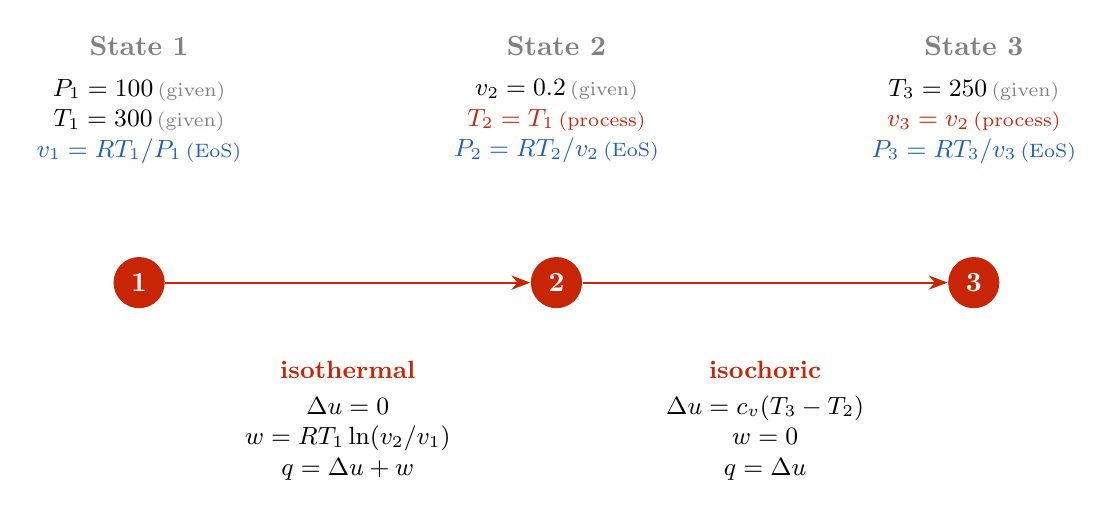
\begin{tikzpicture}[font=\small]
  \node[gray,font=\bfseries] at (0,3.0){State 1};
  \node[gray,font=\bfseries] at (5.3,3.0){State 2};
  \node[gray,font=\bfseries] at (10.6,3.0){State 3};
  \node[align=center] at (0,2.05){\Dg{P_1=100}\\ \Dg{T_1=300}\\ \De{v_1=RT_1/P_1}};
  \node[align=center] at (5.3,2.05){\Dg{v_2=0.2}\\ \Dp{T_2=T_1}\\ \De{P_2=RT_2/v_2}};
  \node[align=center] at (10.6,2.05){\Dg{T_3=250}\\ \Dp{v_3=v_2}\\ \De{P_3=RT_3/v_3}};
  \node[scir] (s1) at (0,0){1};
  \node[scir] (s2) at (5.3,0){2};
  \node[scir] (s3) at (10.6,0){3};
  \draw[pa] (s1) -- (s2);
  \draw[pa] (s2) -- (s3);
  \node[align=center] at (2.65,-1.75){\textcolor{procred}{\textbf{isothermal}}\\[2pt]
    $\Delta u=0$\\ $w=RT_1\ln(v_2/v_1)$\\ $q=\Delta u+w$};
  \node[align=center] at (7.95,-1.75){\textcolor{procred}{\textbf{isochoric}}\\[2pt]
    $\Delta u=\cv(T_3-T_2)$\\ $w=0$\\ $q=\Delta u$};
\end{tikzpicture}
\end{center}

Read the middle column: $v_2$ is \textcolor{gray}{given}, $T_2$ is handed over by
the \textcolor{procred}{process}, and the \textcolor{stateblue}{equation of state}
closes it. That is the pattern the whole method is built to make automatic.

\subsection*{Step 3 \textemdash{} the P\,--\,v sketch}

Sketch the path on a pressure\,--\,volume diagram. The arrow diagram fixed the
\emph{topology} (the order of states); the P\,--\,v sketch shows the \emph{shape}
of each path and checks that the processes join up sensibly. Remember the
boundary work of each process is the area under its curve.

\begin{center}
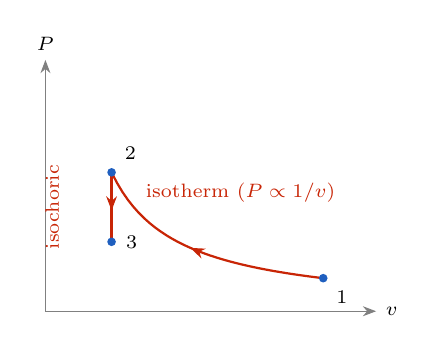
\begin{tikzpicture}[x=0.42cm,y=0.42cm,>=Stealth]
  \draw[->,gray] (0,0)--(10.0,0) node[right,black,font=\scriptsize]{$v$};
  \draw[->,gray] (0,0)--(0,7.6) node[above,black,font=\scriptsize]{$P$};
  \draw[pvc] plot[domain=0:1,samples=40,variable=\t] ({8.4+(2-8.4)*\t},{8.4/(8.4+(2-8.4)*\t)});
  \draw[pvc] (2,4.2)--(2,2.1);
  \node[pvdot,label={[font=\scriptsize]below right:1}] at (8.4,1){};
  \node[pvdot,label={[font=\scriptsize]above right:2}] at (2,4.2){};
  \node[pvdot,label={[font=\scriptsize]right:3}] at (2,2.1){};
  \node[font=\scriptsize,text=procred] at (5.9,3.6){isotherm ($P \propto 1/v$)};
  \node[font=\scriptsize,text=procred,rotate=90,anchor=south] at (0.7,3.15){isochoric};
\end{tikzpicture}
\end{center}

\subsection*{Stage 1 \textemdash{} fix P, v, T at every state}

Now the calculation, in two stages. Stage~1 fixes $P$, $v$, $T$ at every state.
Start at the state where you already know two of the three; the ideal-gas EoS
gives the third. At each next state, the given information supplies one property,
the process supplies a second, and the EoS gives the third. Do not put in numbers
yet \textemdash{} just write the equation under each state (that is what the arrow
diagram already did).

\emph{For our example}, carrying the numbers through:
\[ v_1 = \frac{RT_1}{P_1} = \frac{0.287\times300}{100} = 0.861~\mcube/\text{kg},
   \qquad
   P_2 = \frac{RT_2}{v_2} = \frac{0.287\times300}{0.2} = 430.5~\text{kPa}, \]
\[ P_3 = \frac{RT_3}{v_3} = \frac{0.287\times250}{0.2} = 358.8~\text{kPa}. \]

\subsection*{Stage 2 \textemdash{} $\Delta u$, work and heat for every process}

With $P$, $v$, $T$ known, the energies follow. For every process, three
equations: the internal-energy change $\Delta u = \cv\,\Delta T$; the boundary
work $\wb = \int P\,dv$ along that path; and the heat $q = \Delta u + \wb$. The
only equation that differs between processes is the boundary work:

\begin{center}
\begin{tabular}{@{}ll@{}}
constant volume & $\wb = 0$ \\
constant pressure & $\wb = P\,\Delta v$ \\
isothermal & $\wb = RT_1\ln(v_2/v_1)$ \\
isentropic & $\wb = \cv\,(T_1 - T_2)$ \\
\end{tabular}
\end{center}

\emph{For our example:}
\[ w_{12} = RT_1\ln\frac{v_2}{v_1}
   = 0.287\times300\times\ln\frac{0.2}{0.861} = -125.7~\text{kJ/kg} = q_{12}
   \quad(\Delta u_{12}=0), \]
\[ w_{23} = 0, \qquad
   q_{23} = \Delta u_{23} = \cv(T_3 - T_2) = 0.718\times(250-300)
   = -35.9~\text{kJ/kg}. \]

\subsection*{Finish}

Add the legs together, keeping their signs. The net work is the sum of the
boundary works; the net heat is the sum of the heats. From there you can get
anything else the problem asks.
\[ w_\text{net} = -125.7 + 0 = \boxed{-125.7~\text{kJ/kg}}, \qquad
   q_\text{net} = -125.7 - 35.9 = \boxed{-161.6~\text{kJ/kg}}. \]
Both negative: work is done \emph{on} the gas, heat is rejected \emph{from} it.
A good habit is one self-check across the whole path:
$q_\text{net} - w_\text{net} = \Delta u_{13} = \cv(T_3 - T_1)
= 0.718\times(-50) = -35.9$, and indeed $-161.6 - (-125.7) = -35.9$. \checkmark

% ======================================================================
\section{The plan in one line}

\begin{aside}{monashred}
Identify the ideal gas $\to$ find the states and processes $\to$ draw the arrow
diagram $\to$ sketch the P\,--\,v diagram $\to$ fix $P$, $v$, $T$ at every state
$\to$ then $\Delta u$, work and heat for every process $\to$ finish.
\end{aside}

The same five buckets and the same steps handle any Perfect-Ideal-Gas problem,
whether it is an engine, a pneumatic system, or a full cycle. The planning does
the hard part; the arithmetic that follows is just bookkeeping.

\vfill
\begin{center}\footnotesize\color{gray}
Companion videos, slides and transcripts:
\url{https://rpgroup-monash.github.io/teaching/art-of-solving/}
\end{center}

\end{document}
